\documentclass[aspectratio=169,mathserif]{beamer}
%\documentclass[aspectratio=169,mathserif,handout]{beamer}


\usepackage{graphicx} % Allows including images
\graphicspath{{./img/}}

\usepackage{epstopdf}
\epstopdfsetup{outdir=./img/}

\usepackage[utf8]{inputenc}
%Load useful packages
\usepackage{booktabs} % Allows the use of \toprule, \midrule and \bottomrule in tables
\usepackage{subcaption}
\usepackage{subfiles}
\usepackage{url}
\usepackage{amssymb}
%
\usepackage{multirow}
\usepackage{mathrsfs} 
%
% align enum description
% \usepackage{enumitem}
% refs
\usepackage[style=authoryear,natbib=true]{biblatex}
\bibliography{references.bib}
%
\usepackage{tikz}
\usepackage{tikz-cd}
\usepackage{tikzscale}
\usetikzlibrary{calc,matrix,chains,positioning,decorations.pathreplacing,decorations.text,arrows,cd}

% overlays
\tikzset{
invisible/.style={opacity=0},
visible on/.style={alt={#1{}{invisible}}},
alt/.code args={<#1>#2#3}{%
\alt<#1>{\pgfkeysalso{#2}}{\pgfkeysalso{#3}} % \pgfkeysalso doesn't change the path
},
}

% neural nets
\tikzset{%
  every neuron/.style={
circle,
draw,
%minimum size=1cm
  },
  neuron missing/.style={
draw=none, 
scale=1,
text height=0.333cm,
execute at begin node=\color{black}$\vdots$
  },
}

% infrastructure
\tikzset{
vertex/.style = {
circle,
fill= black,
outer sep = 2pt,
inner sep = 1pt,
}
}




%Information to be included in the title page:
\title{Deep Learning}

\author{Tiago Vieira}
\institute{Institute of Computing\\Universidade Federal de Alagoas}
\date{\today}
%Logo in every slide
%\logo{%
%  \makebox[0.98\paperwidth]{
%\includegraphics[width=0.5cm,keepaspectratio]{../logos/ufal_logo.png}%
%\hfill%\includegraphics[height=1cm,keepaspectratio]{logos/edge_logo.png}%
%\includegraphics[height=0.8cm,keepaspectratio]{../logos/ic_logo.png}%
%  }
%}
%Contents before every section's starting slide
\AtBeginSubsection[]
{
  \begin{frame}
\frametitle{Summary}
\scriptsize
\tableofcontents[currentsection,currentsubsection]
  \end{frame}


}
% shape, colour of item, nested item bullets in itemize only
% \setbeamertemplate{itemize item}[square] \setbeamercolor{itemize item}{bg=blue}
% \setbeamertemplate{itemize subitem}[circle] \setbeamercolor{itemize subitem}{fg=green}
% \setbeamertemplate{itemize subsubitem}[triangle] \setbeamercolor{itemize subsubitem}{fg=red}
% font size of nested and nested-within-nested bulltes in both itemize and enumerate
% options are \tiny, \small, \scriptsize, \normalsize, \footnotesize, \large, \Large, \LARGE, \huge and \Huge
\setbeamerfont{itemize/enumerate subbody}{size=\scriptsize} 
\setbeamerfont{itemize/enumerate subsubbody}{size=\scriptsize}
% figure numbers
% \setbeamertemplate{caption}[numbered]
% blocks style
\setbeamertemplate{blocks}[rounded][shadow=true]


% Hide nav control
\usenavigationsymbolstemplate{}
% add numbering
%\addtobeamertemplate{navigation symbols}{}{%
%\usebeamerfont{footline}%
%\usebeamercolor[fg]{footline}%
%\hspace{1em}%
%\insertframenumber/\inserttotalframenumber
%}

% Footnote without number
\newcommand\blfootnote[1]{%
\begingroup
\renewcommand\thefootnote{}\footnote{#1}%
\addtocounter{footnote}{-1}%
\endgroup
}

% items symbols
\setbeamertemplate{itemize subitem}{-}
\setbeamertemplate{itemize subsubitem}{-}

%%setting up some useful slide creation commands
%split slide
% \newenvironment{splitframe}[5]
% %[1] ==> 1 parameter passed through {}
% %[2] ==> 2 parameters passed through {}{}
% %[4] ==> 4 parameters passed through {}{}{}{}
% {
% \begin{frame}{#3}
% \begin{columns}
% \column{#1\linewidth}
% \centering
% #4
% \column{#2\linewidth}
% \centering
% #5
% \end{columns}
% \centering
% \vspace{\baselineskip} % adds one line space
% }
% %Inside the first pair of braces (ABOVE) is set what your new environment will do before the text within, then inside the second pair of braces (BELOW) declare what your new environment will do after the text. Note second pair can be empty braces too.
% {
% \end{frame}


% }

%\usepackage{calligra}
%\DeclareMathAlphabet{\mathcalligra}{T1}{calligra}{m}{n}


\usepackage{svg}
\usepackage{PSTricks}

\subtitle{Machine Learning with Shallow Neural Networks}

\begin{document}

\frame{\titlepage}

\begin{frame}
\frametitle{Summary}
{\tableofcontents}
\end{frame}

\section{Introduction}

\begin{frame}{Neural Networks and Machine Learning}
\begin{itemize}
\item Neural networks are optimization-based learning models.
\item  Many classical machine learning models  use
continuous optimization:
\begin{itemize}
\item SVMs, Linear Regression, and Logistic Regression
\item Singular Value Decomposition
\item (Incomplete) Matrix factorization for Recommender Systems
\end{itemize}
\item All these models can be represented as special cases of shallow neural
networks!
\end{itemize}
\end{frame}

\begin{frame}{The Continuum Between Machine Learning and Deep Learning}
\begin{center}
\includegraphics[width=.4\textwidth]{comparison.eps}
\end{center}
\begin{itemize}
\item Classical machine learning models
 reach their learning capacity early because they are simple neural networks.
\item When we have more data, we can add more computational units to
improve performance.
\end{itemize}
\end{frame}


\begin{frame}{The Deep Learning Advantage}
\begin{itemize}
\item Exploring the neural models for traditional machine learning
is useful because it exposes the cases in which deep learning has an
advantage.
\begin{itemize}
\item Add capacity with more nodes for more data.
\item Controlling the structure of the architecture provides a way
to incorporate domain-specific insights (e.g., recurrent networks
and convolutional networks).
\end{itemize}
\item In some cases, making minor changes to the architecture leads
to interesting models:
\begin{itemize}
\item Adding a sigmoid/softmax layer in the output of a neural model
for (linear) matrix factorization can result in logistic/multinomial
matrix factorization (e.g., word2vec).
\end{itemize}
\end{itemize}
\end{frame}


\begin{frame}{}
\centering
\begin{block}{}
\textit{Is deep learning simply a stacking of simpler models like logistic or linear regression}?
\end{block}
\end{frame}

\begin{frame}{}
\centering
\begin{block}{}
\textit{Domain-Specific understanding:}
\begin{itemize}
\item Convolutional neural networks.
\item Recurrent neural networks.
\end{itemize}
\end{block}
\end{frame}


%As a specific example, the loss function of the L2-support vector machine was proposed by Hinton [190] in the context of a neural architecture in 1989. When used with regularization, the resulting neural network would behave identically to an L2-support vector machine. In comparison, Cortes and Vapnik’s paper on the support vector machine [82] appeared several years later with an L1-loss function. These relationships are not surprising because the best way to define a shallow neural network is often closely related to a known machine learning algorithm. Therefore, it is important to explore these basic neural models in order to develop an integrated view of neural networks and traditional machine learning.

% Como um exemplo específico, a função de perda da máquina de vetor de suporte L2 foi proposta por Hinton [190] no contexto de uma arquitetura neural em \textbf{1989} (Connectionist Learning Procedures). Quando usada com regularização, a rede neural resultante se comportaria de forma idêntica a um vetor de suporte L2 máquina. Em comparação, o artigo de Cortes e Vapnik sobre a máquina de vetores de suporte [82] apareceu vários anos depois com uma função de perda L1. Esses relacionamentos não são surpreendentes porque a melhor maneira de definir uma rede neural superficial está frequentemente relacionada a um algoritmo de aprendizado de máquina conhecido. Portanto, é importante explorar esses modelos neurais básicos para desenvolver uma visão integrada das redes neurais e do aprendizado de máquina tradicional.

\section{Neural Architectures for Binary Classification Models}



\begin{frame}{Recap: Perceptron versus Linear Support Vector Machine}
 \begin{tabular}{cc}
\includegraphics[width=.45\textwidth]{neuralvary2.eps}&
\includegraphics[width=.45\textwidth]{neuralvary6.eps}\\
(a) Perceptron & (b) SVM  \\
 Loss $= \mbox{max}\{ 0, -y (\overline{W} \cdot \overline{X}) \}$
&    Loss $= \mbox{max}\{ 0, 1-y (\overline{W} \cdot \overline{X})
\}$
\end{tabular}
\begin{itemize}
\item The Perceptron criterion is a minor variation of hinge loss with identical update of $\overline{W}  \Leftarrow  \overline{W} +  \alpha  y
\overline{X}$ in both cases.
\item We update only for misclassified instances in perceptron, but update {\em also} for
``marginally correct'' instances in SVM.
\end{itemize}
\end{frame}


\begin{frame}{Perceptron Criterion versus Hinge Loss}
\begin{center}
\includegraphics[width=.6\textwidth]{hingevsp}
\end{center}
\begin{itemize}
\item Loss for positive class training instance at varying values of
$\overline{W}\cdot \overline{X}$.
\end{itemize}
\end{frame}


\begin{frame}{What About the Kernel SVM?}
%\begin{center}
%\includegraphics[scale=0.85]{../rbf/rbf.eps}
%\end{center}
\begin{itemize}
\item RBF Network for unsupervised feature engineering.
\begin{itemize}
\item Unsupervised feature engineering is good for noisy data.
\item Supervised feature engineering (with deep learning) is good
for learning rich structure. \end{itemize}
\end{itemize}
\end{frame}


\begin{frame}{Much of Machine Learning is a Shallow Neural Model}
\begin{itemize}
\item  By minor changes to the architecture of  perceptron we can get:
\begin{itemize}
\item Linear regression, Fisher discriminant, and Widrow-Hoff learning $\Rightarrow$ Linear activation in output
node
\item Logistic regression $\Rightarrow$ Sigmoid activation in output
node
\end{itemize}
\item Multinomial logistic regression $\Rightarrow$ Softmax
Activation in Final Layer
\item Singular value decomposition $\Rightarrow$ Linear autoencoder
\item Incomplete matrix factorization for Recommender Systems  $\Rightarrow$ Autoencoder-like architecture  with
single hidden layer (also used in {\em word2vec})
\end{itemize}
\end{frame}


\begin{frame}{Why do We Care about Connections?}
\begin{itemize}
\item Connections tell us about the cases that it makes sense to use
conventional machine learning:
\begin{itemize}
\item If you have less data with noise, you want to use conventional
machine learning.
\item If you have a lot of data with rich structure, you want to use
neural networks.
\item Structure is often learned by using deep neural
architectures.
\end{itemize}
\item Architectures like convolutional neural networks can use
domain-specific insights.
\end{itemize}
\end{frame}




\begin{frame}{Widrow-Hoff Rule: The Neural Avatar of Linear
Regression}
\begin{itemize}
\item  The perceptron (1958) was historically followed by  Widrow-Hoff
Learning (1960).
\item Identical to linear regression when applied to
numerical targets.
\begin{itemize}
\item  Originally proposed by Widrow and Hoff for binary targets (not natural for regression).
\end{itemize}
\item The Widrow-Hoff method, when applied to
mean-centered features and mean-centered binary class encoding,
learns the   Fisher discriminant.
\item We first discuss linear regression for numeric classes and
then visit the case of binary classes.
\end{itemize}
\end{frame}


\begin{frame}{Linear Regression: An Introduction}
\begin{itemize}
\item In linear regression, we have training pairs $(\overline{X}_i,
y_i)$ for $i \in \{ 1 \ldots n \}$, so that $\overline{X_i}$
contains $d$-dimensional features and $y_i$ contains a numerical
target.
\item We use a linear parameterized function to  predict $\hat{y}_i= \overline{W} \cdot
\overline{X}_i$.
\item Goal is to  learn $\overline{W}$, so that the sum-of-squared differences
between observed  $y_i$ and predicted $\hat{y}_i$ is minimized over
the entire training data.
\item Solution exists in closed form, but requires the inversion of a potentially large
matrix. \item  Gradient-descent is typically used anyway.
\end{itemize}
\end{frame}


\begin{frame}{Linear Regression with Numerical Targets:Neural Model}
\begin{center}
\includegraphics[width=.6\textwidth]{neuralvary3.eps}
\end{center}
\begin{itemize}
\item Predicted output is $\hat{y}_i= \overline{W}\cdot \overline{X}_i$ and loss is $L_i=(y_i -\hat{y}_i)^2$.
\item  Gradient-descent update is $\overline{W} \Leftarrow
\overline{W} - \alpha \frac{\partial L_i}{\partial \overline{W}} =
\overline{W}+ \alpha (y_i - \hat{y}_i) \overline{X}_i$.
\end{itemize}
\end{frame}


\begin{frame}{Widrow-Hoff: Linear Regression with Binary Targets}
\begin{itemize}
\item For  $y_i \in \{-1,
+1 \}$, we use  same loss of $(y_i -\hat{y}_i)^2$, and update of
$\overline{W} \Leftarrow
 \overline{W}+ \alpha \underbrace{(y_i - \hat{y}_i)}_{\mbox{delta}} \overline{X}_i$.
 \begin{itemize}
 \item When applied to binary targets, it is referred to as delta
 rule.
 \item Perceptron uses the same update with $\hat{y}_i= \mbox{sign} \{
 \overline{W} \cdot \overline{X}_i \}$, whereas Widrow-Hoff uses
 $\hat{y}_i= \overline{W} \cdot \overline{X}_i$.
 \end{itemize}
 \item {\bf Potential drawback:} Retrogressive treatment of
 well-separated points caused by the pretension  that binary targets are real-valued.
 \begin{itemize}
\item If $y_i=+1$, and $\overline{W} \cdot \overline{X}_i =10^6$,
the point will be heavily penalized for strongly correct
classification!
\item Does not happen in perceptron.
\end{itemize}
 \end{itemize}
\end{frame}


\begin{frame}{Comparison of Widrow-Hoff with Perceptron and SVM}
\begin{itemize}
\item Convert the binary loss functions and updates to a form more
easily comparable to perceptron using $y_i^2=1$:
\item Loss of $(\overline{X}_i, y_i)$ is  $(y_i -\overline{W} \cdot
\overline{X}_i)^2 = (1 - y_i [\overline{W}\cdot
\overline{X}_i])^2$\\
Update: $\overline{W} \Leftarrow  \overline{W}+ \alpha y_i
(1-y_i[\overline{W} \cdot \overline{X}_i]) \overline{X}_i$
\end{itemize}
\begin{center}
{\footnotesize
\begin{tabular}{||c||c|c||}
\hline \hline
& Perceptron &  $L_1$-Loss SVM \\
Loss &  $\mbox{max}\{  -y_i (\overline{W}\cdot \overline{X}_i), 0
\}$ & $\mbox{max}\{ 1 -y_i (\overline{W}\cdot
\overline{X}_i), 0 \}$ \\
 Update & $\overline{W} \Leftarrow  \overline{W}+ \alpha y_i
I(-y_i[\overline{W} \cdot \overline{X}_i]>0) \overline{X}_i$  &
$\overline{W} \Leftarrow  \overline{W}+ \alpha y_i
I(1-y_i[\overline{W} \cdot \overline{X}_i]>0) \overline{X}_i$\\
 \hline \hline
\end{tabular}}
\end{center}
\begin{center}
{\footnotesize
\begin{tabular}{||c||c|c|c|c||}
\hline \hline
&  Widrow-Hoff  &  Hinton's $L_2$-Loss SVM\\
 Loss &  $(1 - y_i (\overline{W}\cdot
\overline{X}_i))^2$ & $\mbox{max}\{
1 -y_i (\overline{W}\cdot \overline{X}_i), 0 \}^2$\\
 Update & $\overline{W} \Leftarrow \overline{W}+ \alpha y_i
(1-y_i[\overline{W} \cdot \overline{X}_i]) \overline{X}_i$ &
$\overline{W} \Leftarrow \overline{W}+ \alpha y_i \mbox{max}\{
(1-y_i[\overline{W} \cdot \overline{X}_i]) , 0
\} \overline{X}_i$\\
 \hline \hline
\end{tabular}}
\end{center}
\end{frame}


\begin{frame}{Some Interesting Historical Facts}
\begin{itemize}
\item Hinton proposed the SVM $L_2$-loss three years before Cortes
and Vapnik's paper on SVMs. \begin{itemize}
 \item G. Hinton. Connectionist learning procedures. {\em
Artificial Intelligence}, 40(1--3), pp.~185--234, 1989.
\item Hinton's $L_2$-loss was proposed to address some of the
weaknesses of loss functions like linear regression on binary
targets. \item When used with $L_2$-regularization, it behaves
identically to an $L_2$-SVM, but the connection with SVM was
overlooked.
\end{itemize}
\item The Widrow-Hoff rule is also referred to as ADALINE, LMS
(least mean-square method), delta rule, and least-squares
classification.
\end{itemize}
\end{frame}


\begin{frame}{Connections with Fisher Discriminant}
\begin{itemize}
\item Consider a binary classification problem with training
instances $(\overline{X}_i, y_i)$ and $y_i \in \{ -1, +1 \}$.
\begin{itemize}
\item Mean-center each feature vector as $\overline{X_i} - \overline{\mu}$.
\item Mean-center the binary class by  subtracting $\sum_{i=1}^n
y_i/n$ from each $y_i$.
\end{itemize}
\item Use the delta rule $\overline{W} \Leftarrow
 \overline{W}+ \alpha \underbrace{(y_i - \hat{y}_i)}_{\mbox{delta}} \overline{X}_i$ for
 learning.
\item Learned vector is the Fisher discriminant!
\begin{itemize}
\item Proof in  Christopher Bishop's book on machine learning.
\end{itemize}
\end{itemize}
\end{frame}




\begin{frame}{Logistic Regression: A Probabilistic Model}
\begin{itemize}
\item Consider the training pair $(\overline{X}_i, y_i)$ with
$d$-dimensional feature variables in $\overline{X_i}$ and class
variable $y_i \in \{ -1, +1 \}$.
\item In logistic regression, the sigmoid function is applied to
$\overline{W} \cdot \overline{X}_i$, which predicts  the probability
that  $y_i$ is $+1$.
\begin{equation*}
\hat{y}_i= P(y_i=1)= \frac{1}{1 +\mbox{exp}(-\overline{W} \cdot
\overline{X}_i)}
\end{equation*}
\item  We want to {\em maximize} $\hat{y}_i$ for positive class instances
and $1- \hat{y}_i$ for negative class instances.
\begin{itemize}
\item Same as {\em minimizing} $-\mbox{log}(\hat{y}_i)$ for positive
class instances and $-\mbox{log}(1- \hat{y}_i)$ for negative
instances.
\item Same as minimizing loss $L_i=-\mbox{log}(|y_i/2 -0.5 + \hat{y}_i |)$.
\item Alternative form of loss $L_i= \mbox{log}(1+ \mbox{exp}[-y_i( \overline{W} \cdot \overline{X}_i)])$
\end{itemize}
\end{itemize}
\end{frame}


\begin{frame}{Maximum-Likelihood Objective Functions}
\begin{itemize}
\item Why did we use the negative logarithms?
\item Logistic regression is an example of a maximum-likelihood
objective function.
\item Our goal is to maximize the {\em product} of the probabilities of
 correct classification over all training instances.
 \begin{itemize}
 \item Same as minimizing the {\em sum} of the negative log probabilities.
 \item Loss functions are always {\em additive} over training
 instances.
 \item So we are really minimizing $\sum_i -\mbox{log}(|y_i/2 -0.5 + \hat{y}_i
 |)$ which can be shown to be $\sum_i \mbox{log}(1+ \mbox{exp}[-y_i( \overline{W} \cdot \overline{X}_i)])$.
 \end{itemize}
\end{itemize}
\end{frame}


\begin{frame}{Logistic Regression: Neural Model}
\begin{center}
\includegraphics[width=.5\textwidth]{neuralvary4.eps}
\end{center}
\begin{itemize}
\item Predicted output is $\hat{y}_i=  1/(1 +\mbox{exp}(-\overline{W} \cdot
\overline{X}_i))$ and loss is $L_i= -\mbox{log}(|y_i/2 -0.5 +
\hat{y}_i
 |) = \mbox{log}(1+ \mbox{exp}[-y_i( \overline{W} \cdot \overline{X}_i)]) $.
 \begin{itemize}
\item  Gradient-descent update is $\overline{W} \Leftarrow
\overline{W} - \alpha \frac{\partial L_i}{\partial \overline{W}}$.
\begin{equation*}
\overline{W} \Leftarrow \overline{W}+ \alpha \frac{y_i
\overline{X_i}}{1 + \mbox{exp}[y_i (\overline{W}\cdot
\overline{X_i})]} \end{equation*}
\end{itemize}
\end{itemize}
\end{frame}


\begin{frame}{Interpreting the Logistic Update}
 \begin{itemize}
 \item An important multiplicative  factor in the update increment is $1/(1+
 \mbox{exp}[y_i(\overline{W}\cdot \overline{X}_i)])$.
 \item This factor is $1-\hat{y}_i$ for positive instances and
 $\hat{y}_i$ for negative instances $\Rightarrow$ Probability of
 mistake!
 \item Interpret as: $\overline{W} \Leftarrow \overline{W}+ \alpha \left[ \mbox{Probability of mistake on
$(\overline{X_i}, y_i)$} \right] \, (y_i \overline{X_i})$
\end{itemize}
\end{frame}


\begin{frame}{Comparing Updates of Different Models}
\begin{itemize}
\item The unregularized updates of the perceptron, SVM, Widrow-Hoff, and logistic
regression can all be written in the following form:
\begin{equation*}
\overline{W} \Leftarrow \overline{W} +  \alpha y_i
\delta(\overline{X}_i, y_i) \overline{X}_i
\end{equation*}
\item The quantity $\delta(\overline{X}_i, y_i)$ is a {\em mistake
function}, which is:
\begin{itemize}
\item Raw mistake value $(1- y_i (\overline{W}\cdot \overline{X}_i))$ for Widrow-Hoff
\item Mistake indicator whether  $(0- y_i (\overline{W}\cdot
\overline{X}_i))>0$ for perceptron.
\item Margin/mistake indicator whether $(1- y_i (\overline{W}\cdot
\overline{X}_i))>0$ for SVM.
\item Probability of mistake on $(\overline{X}_i, y_i)$ for logistic
regression.
\end{itemize}
\end{itemize}
\end{frame}


\begin{frame}{Comparing Loss Functions of Different Models}
\begin{center}
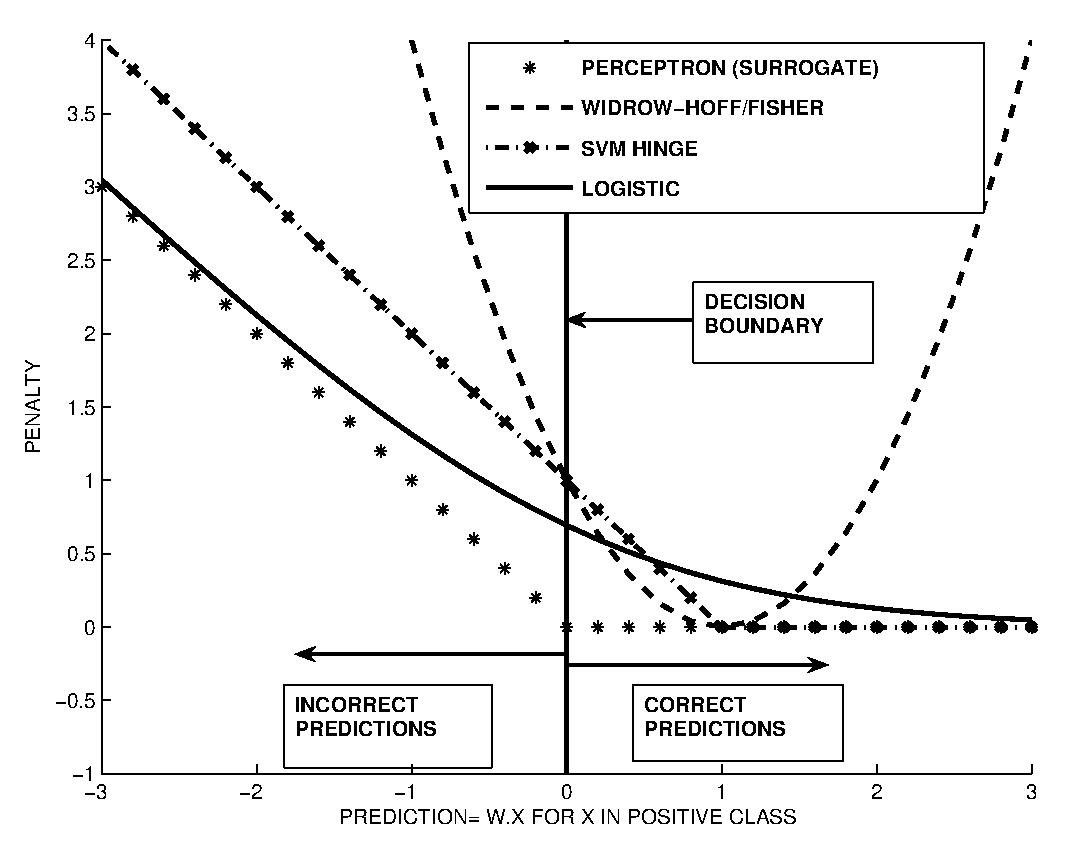
\includegraphics[width=.5\textwidth]{lossfunc.eps}
\end{center}
\begin{itemize}
\item Loss
functions are  similar (note  Widrow-Hoff retrogression).
\end{itemize}
\end{frame}


\begin{frame}{Other Comments on Logistic Regression} \begin{itemize}
\item Many classical neural models use repeated  computational units with  logistic and tanh
activation functions in hidden layers.
\item One can view these methods as feature engineering models that
stack multiple logistic regression models.
\item The stacking of multiple models creates inherently more
powerful models than their individual components.
\end{itemize}
\end{frame}



\begin{frame}{Binary Classes versus Multiple Classes}
\begin{itemize}
\item All the models discussed so far discuss only the binary class
setting in which the class label is drawn from $\{ -1, +1 \}$.
\item Many natural applications contain  multiple classes without a natural ordering among them:
\begin{itemize}
\item Predicting the category of an image (e.g., {\em truck},
{\em carrot}).
\item {\em Language models:} Predict the next word in a sentence.
\end{itemize}
\item Models like logistic regression are naturally designed to predict two classes.
\end{itemize}
\end{frame}


\begin{frame}{Generalizing Logistic Regression}
\begin{itemize}
\item Logistic regression produces probabilities of the two outcomes
of a binary class.
\item {\em Multinomial} logistic regression  produces probabilities
of multiple outcomes.
\begin{itemize}
\item In order to produce probabilities of multiple classes, we need
an activation function with a vector output of probabilities.
\item The {\em softmax activation function} is a vector-based
generalization of the sigmoid activation used in logistic
regression.
\end{itemize}
\item Multinomial logistic regression is also referred to as softmax classifier.
\end{itemize}
\end{frame}


\begin{frame}{The Softmax Activation Function}
\begin{itemize}
\item The softmax activation function is a natural vector-centric
generalization of the scalar-to-scalar sigmoid activation
$\Rightarrow$ vector-to-vector function.
\item Logistic sigmoid activation: $\Phi(v)= 1/(1+ \mbox{exp}(-v))$.
\item Softmax activation: $\Phi(v_1 \ldots v_k)= \frac{1}{\sum_{i=1}^k \mbox{exp}(v_i)}
\left[ \mbox{exp}(v_1) \ldots \mbox{exp}(v_k) \right]$
\begin{itemize}
\item The  $k$ outputs (probabilities) sum to 1.
\end{itemize}
\item Binary case of using sigmoid$(v)$ is identical to using
2-element  softmax activation with arguments $(v, 0)$.
\begin{itemize}
\item Multinomial logistic regression with 2-element softmax is
equivalent to binary logistic regression.
\end{itemize}
\end{itemize}
\end{frame}


\begin{frame}{Loss Functions for Softmax}
\begin{itemize}
\item Recall that we use the negative logarithm of the probability
of observed class in binary logistic regression.
\begin{itemize}
\item Natural generalization to multiple classes.
\item Cross-entropy loss: Negative logarithm of the probability of
correct class.
\item Probability distribution among incorrect classes has no
effect.
\end{itemize}
\item Softmax activation is used almost exclusively in output layer
and (almost) always  paired with cross-entropy loss.
\end{itemize}
\end{frame}


\begin{frame}{Cross-Entropy Loss of Softmax}
\begin{itemize}
\item Like the binary logistic case, the loss $L$ is a negative log
probability.
\begin{align*}
& \mbox{Softmax Probability Vector} \Rightarrow [\hat{y}_1, \hat{y}_2, \ldots \hat{y}_k]\\
& [\hat{y}_1 \ldots \hat{y}_k]= \frac{1}{\sum_{i=1}^k
\mbox{exp}(v_i)} \left[ \mbox{exp}(v_1) \ldots \mbox{exp}(v_k)
\right]
\end{align*}
 \item The loss is  $-\mbox{log}(\hat{y}_c)$, where $c \in \{
1 \ldots k \}$ is the correct class of that training instance.
\item Cross entropy loss is  $ -v_{c)} + \mbox{log}[\sum_{j=1}^k
\mbox{exp}(v_j)]$
\end{itemize}
\end{frame}


\begin{frame}{Loss Derivative of Softmax}
\begin{itemize}
\item Since softmax is almost always paired with cross-entropy loss
$L$, we can directly estimate $\frac{\partial L}{\partial v_r}$ for
each pre-activation value from $v_1 \ldots v_k$.
\item  Differentiate loss value of  $ -v_{c} + \mbox{log}[\sum_{j=1}^k
\mbox{exp}(v_j)]$
\item Like the sigmoid derivative, the result is best expressed in
terms of the post-activation values $\hat{y}_1 \ldots \hat{y}_k$.
\item The  loss derivative of the softmax is as follows:
\begin{equation*}
\frac{\partial L}{\partial v_r}= \begin{cases} \hat{y}_r -1 &
\mbox{If $r$ is
correct class}\\
\hat{y}_r & \mbox{If $r$ is not correct class}
\end{cases}
\end{equation*}
\end{itemize}
\end{frame}


\begin{frame}{Multinomial Logistic Regression}
\begin{center}
\includegraphics[scale=0.4]{multi3.eps}
\end{center}
\begin{itemize}
\item The $i$th training instance is $(\overline{X}_i, c(i))$,
where $c(i) \in \{ 1 \ldots k\}$ is class index $\Rightarrow$ Learn
$k$ parameter vectors $\overline{W}_1 \ldots \overline{W}_k$.
\begin{itemize}
\item
Define real-valued score $v_r = \overline{W}_r \cdot \overline{X}_i$
for $r$th class.
\item Convert scores to probabilities $\hat{y}_1 \ldots \hat{y}_k$ with softmax activation on
$v_1 \ldots v_k$ $\Rightarrow$ Hard or soft prediction
\end{itemize}
\end{itemize}
\end{frame}


\begin{frame}{Computing the Derivative of the Loss}
\begin{itemize}
\item The cross-entropy loss for the $i$th training instance is
$L_i=-\mbox{log}(\hat{y}_{c(i)})$.
\item For gradient-descent, we need to compute $\frac{\partial
L_i}{\partial \overline{W}_r}$.
\item Using chain rule of differential calculus, we get:
\begin{align*}
\frac{\partial L_i}{\partial \overline{W_r}} &=\sum_j  \left( \frac{\partial L_i}{\partial v_j} \right) \left( \frac{\partial v_j}{\partial \overline{W_r}} \right) = \frac{\partial L_i}{\partial v_r} \underbrace{\frac{\partial v_r}{\partial \overline{W_r}}}_{\overline{X_i}} + \mbox{Zero-terms} \\
 &= \begin{cases}
-\overline{X_i}(1 -\hat{y}_r) & \mbox{ if $r= c(i)$}\\
\overline{X_i} \, \hat{y}_r & \mbox{ if $r \not=c(i)$}
\end{cases} \label{2softgrad}
\end{align*}
\end{itemize}
\end{frame}


\begin{frame}{Gradient Descent Update}
\begin{itemize}
\item Each separator $\overline{W_r}$ is updated using the gradient:
\begin{equation*}
\overline{W_r} \Leftarrow \overline{W_r} - \alpha \frac{\partial
L_i}{\partial \overline{W_r}}
\end{equation*}
\item Substituting the gradient from the previous slide, we obtain:
\begin{equation*}
\overline{W_r} \Leftarrow \overline{W_r}  + \alpha
\begin{cases}
\overline{X_i} \cdot (1 - \hat{y}_r) & \mbox{ if $r= c(i)$}\\
-\overline{X_i} \cdot \hat{y}_r & \mbox{ if $r \not=c(i)$}
\end{cases}
\end{equation*}
\end{itemize}
\end{frame}




\begin{frame}{Unsupervised Learning}
\begin{itemize}
\item The models we have discussed so far use training pairs of the
form $(\overline{X}, y)$ in which the feature variables
$\overline{X}$ and target $y$ are clearly separated.
\begin{itemize}
\item The target variable $y$ provides the {\em supervision} for the
learning process.
\end{itemize}
\item What happens when we do not have a target variable?
\begin{itemize}
\item We want to capture a model of the
training data without the guidance of the target. \item This is an
{\em unsupervised} learning problem.
\end{itemize}
\end{itemize}
\end{frame}


\begin{frame}{Example}
\begin{itemize}
\item Consider a 2-dimensional data set in which all points are
 distributed on the circumference of an origin-centered circle.
\item All points in the first and third quadrant belong to class
$+1$ and remaining points are $-1$.
\begin{itemize}
\item The class variable provides focus to the learning process of the supervised model.
\item An unsupervised model needs  to recognize the
circular manifold without being told up~front.
\item The unsupervised model can represent the data in only 1
dimension (angular position).
\end{itemize}
\item Best way of modeling is data-set dependent $\Rightarrow$ Lack
of supervision causes problems
\end{itemize}
\end{frame}


\begin{frame}{Unsupervised Models and Compression}
\begin{itemize}
\item Unsupervised models are closely related to compression because compression
captures a model of regularities in the data.
\begin{itemize}
\item Generative models represent the data in terms of a compressed
parameter set.
\item Clustering models represent the data in terms of cluster
statistics. \item Matrix factorization represents data in terms of
low-rank approximations (compressed matrices).
\end{itemize}
\item An autoencoder also provides a compressed representation of
the data.
\end{itemize}
\end{frame}


\begin{frame}{Defining the Input and Output of an Autoencoder}
\begin{center}
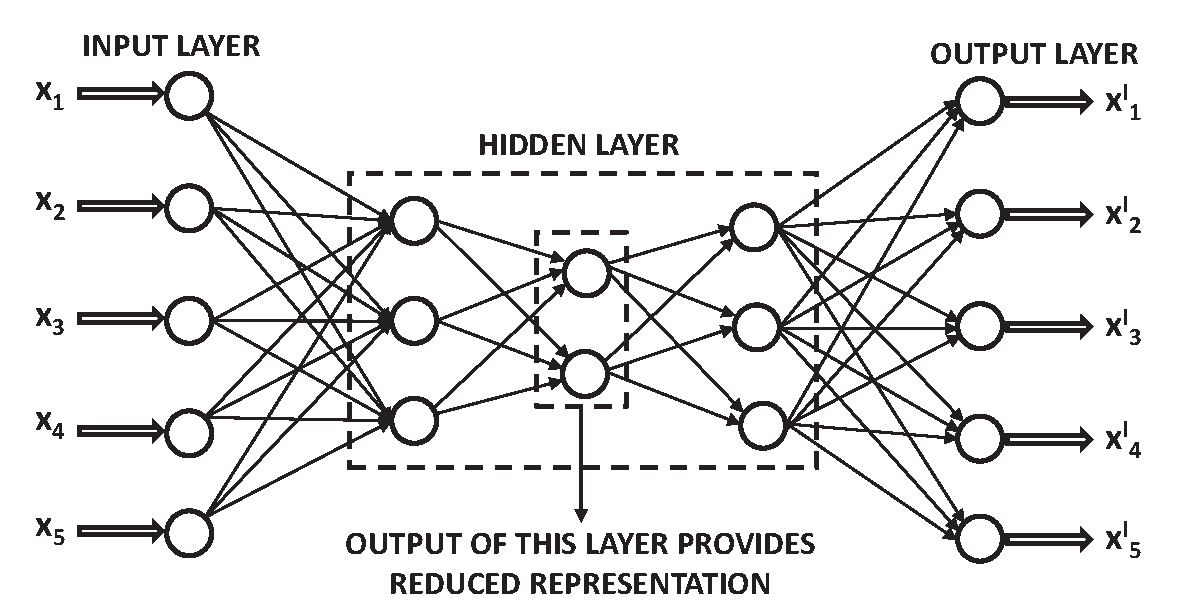
\includegraphics[scale=0.4]{autoencoder.eps}
\end{center}
\begin{itemize}
\item All neural networks work with input-output pairs.
\begin{itemize}
\item In a supervised problem,  the output is the
label.
\end{itemize}
\item In the autoencoder, the output values  are the same as inputs: {\em replicator neural network}.
\begin{itemize}
\item The loss function penalizes a training instance depending on
how far it is from the input (e.g., squared loss).
\end{itemize}
\end{itemize}
\end{frame}


\begin{frame}{Encoder and Decoder}
\begin{center}
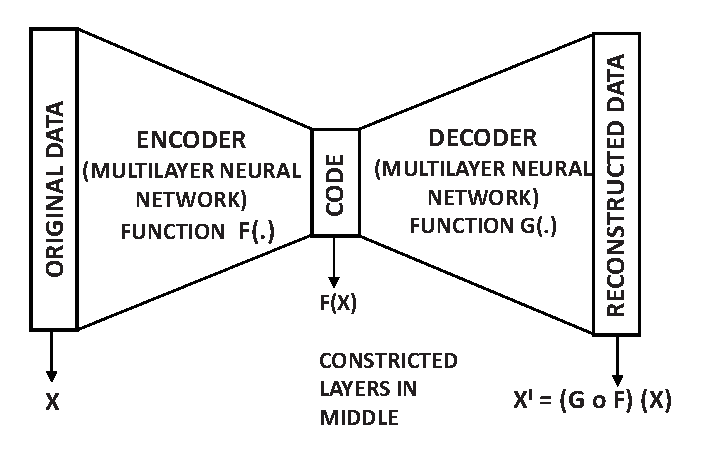
\includegraphics[width=.6\textwidth]{auto.eps}
\end{center}
\begin{itemize}
\item Reconstructing the  data might seem like a trivial matter by
simply copying the data forward from one layer to another.
\begin{itemize}
\item Not
possible when the number of units in the middle are {\em
constricted}.
\item Autoencoder is divided into {\em encoder} and {\em decoder}.
\end{itemize}
\end{itemize}
\end{frame}


\begin{frame}{Basic Structure of Autoencoder}
\begin{itemize}
\item  It is common (but not necessary) for an $M$-layer  autoencoder to have a symmetric
architecture between the input and output.
\begin{itemize}
\item The number of units in the $k$th layer is the same as that in the
$(M-k+1)$th layer.
\end{itemize}
\item The value of $M$ is often odd, as a result of which the $(M+1)/2$th
layer is often the most constricted layer.
\begin{itemize}
\item We are counting the
(non-computational) input layer as the first layer. \item The
minimum number of layers in an autoencoder would be three,
corresponding to the input layer, constricted layer, and the output
layer.
\end{itemize}
\end{itemize}
\end{frame}


\begin{frame}{Undercomplete Autoencoders and Dimensionality
Reduction}
\begin{itemize}
\item The number of units in each middle layer is typically fewer than that in the
input (or output). \begin{itemize} \item These  units hold a reduced
representation of the data, and the final layer can no longer
reconstruct the data exactly.
\end{itemize}
 \item This type of reconstruction
is inherently {\em lossy}.
\item The activations of hidden layers provide an alternative to
linear and nonlinear dimensionality reduction techniques.
\end{itemize}
\end{frame}


\begin{frame}{Overcomplete Autoencoders and Representation Learning}
\begin{itemize}
\item  What happens if the number of units in hidden layer is equal
to or larger than  input/output layers?
\begin{itemize}
\item There are infinitely many  hidden representations with zero error.
\item  The middle layers often do not learn the identity
function.
\item We can  enforce specific properties on
the redundant representations by adding constraints/regularization
to hidden layer.
\begin{itemize}
\item Training with stochastic gradient descent is itself a form of
regularization.
\item One can learn sparse features by adding sparsity constraints to hidden layer.
\end{itemize}
\end{itemize}
\end{itemize}
\end{frame}


\begin{frame}{Applications}
\begin{itemize}
\item Dimensionality reduction $\Rightarrow$ Use activations of
constricted hidden layer
\item Sparse feature learning $\Rightarrow$ Use activations of
constrained/regularized hidden layer
\item Outlier detection: Find data points with larger reconstruction
error
\begin{itemize}
\item Related to denoising applications
\end{itemize}
\item Generative models with probabilistic hidden layers
(variational autoencoders)
\item Representation learning $\Rightarrow$ Pretraining
\end{itemize}
\end{frame}




\begin{frame}{Singular Value Decomposition}
\begin{itemize}
\item Truncated SVD is the {\em approximate} decomposition of an $n \times d$ matrix $D$ into
$D \approx Q \Sigma P^T$, where  $Q$, $\Sigma$, and $P$ are $n
\times k$, $k \times k$, and $d \times k$ matrices, respectively.
\begin{itemize}
\item Orthonormal columns of  each of $P$, $Q$, and nonnegative
diagonal matrix $\Sigma$.
\item Minimize the squared sum of residual entries in $D - Q \Sigma P^T$.
\item The value of $k$ is typically much smaller than  $\mbox{min}\{ n, d
\}$.
\item Setting $k$ to  $\mbox{min}\{ n, d \}$ results in a zero-error decomposition.
\end{itemize}
\end{itemize}
\end{frame}


\begin{frame}{Relaxed and Unnormalized Definition of  SVD}
\begin{itemize}
\item {\bf Two-way Decomposition:} Find an $n \times k$ matrix $U$,  and $d \times k$ matrix $V$ so that $||D
- U V^T||^2$ is minimized.
\begin{itemize}
\item Property: At least one optimal pair $U$ and $V$ will have
mutually orthogonal columns (but non-orthogonal alternatives will
exist).
\item The orthogonal solution can be converted into the 3-way
factorization of SVD.
\item Exercise: Given $U$ and $V$ with orthogonal columns, find $Q$, $\Sigma$ and $P$.
\end{itemize}
\item In the event that $U$ and $V$ have non-orthogonal columns at optimality,
these columns will span the same subspace as the orthogonal solution
at optimality.
\end{itemize}
\end{frame}


\begin{frame}{Dimensionality Reduction and Matrix Factorization}
\begin{itemize}
\item Singular value decomposition is a dimensionality reduction
method (like any matrix factorization technique).
\begin{equation*}
D \approx U V^T
\end{equation*}
\item The $n$ rows of $D$ contain the $n$ training points.
\item The $n$ rows of $U$  provide the reduced representations of
the training points.
\item The $k$ columns of $V$ contain the orthogonal basis vectors.
\end{itemize}
\end{frame}


\begin{frame}{The Autoencoder Architecture for SVD}
\begin{columns}
\begin{column}{.5\textwidth}
\begin{figure}[!]
\centering
\includegraphics[width=\textwidth]{encoder2.eps}
\end{figure}
\end{column}
\begin{column}{.5\textwidth}
\begin{itemize}
\item The rows of matrix $D$ are input to encoder.
\item The activations of hidden layer are rows of $U$ and the
weights of the decoder contain $V$.
\item The reconstructed data contain the rows of $UV^T$.
\end{itemize}
\end{column}
\end{columns}
\end{frame}


\begin{frame}{Why is this SVD?}
\begin{itemize}
\item If we use the mean-squared error as the loss function, we are
optimizing $||D -UV^T||^2$ over the entire training data.
\begin{itemize}
\item This is the same objective function as SVD!
\end{itemize}
\item  It is possible for gradient-descent to arrive at an optimal solution in which
 the columns of each of $U$ and $V$ might not be
mutually orthogonal.
\item Nevertheless, the subspace spanned by the columns of each of
$U$ and $V$ will always be the same as that found by the optimal
solution of SVD.
\end{itemize}
\end{frame}


\begin{frame}{Some Interesting Facts}
\begin{itemize}
\item The optimal encoder weight matrix $W$ will be the pseudo-inverse
of the decoder weight matrix  $V$ if the training data spans the
full dimensionality.
\begin{equation*}
W= (V^T V)^{-1} V^T
\end{equation*}
\begin{itemize}
\item If the encoder and decoder weights are tied $W=V^T$, the columns of
the weight matrix $V$ will  become mutually orthogonal.
\item Easily shown by substituting $W=V^T$ above and postmultiplying with
$V$ to obtain $V^TV=I$.
\item This is exactly SVD!
\end{itemize}
\item Tying encoder-decoder weights does not lead to orthogonality for other architectures, but
is a common practice anyway.
\end{itemize}
\end{frame}


\begin{frame}{Deep Autoencoders}
\begin{columns}[t]
\begin{column}{.5\textwidth}
\begin{figure}[!]
\centering
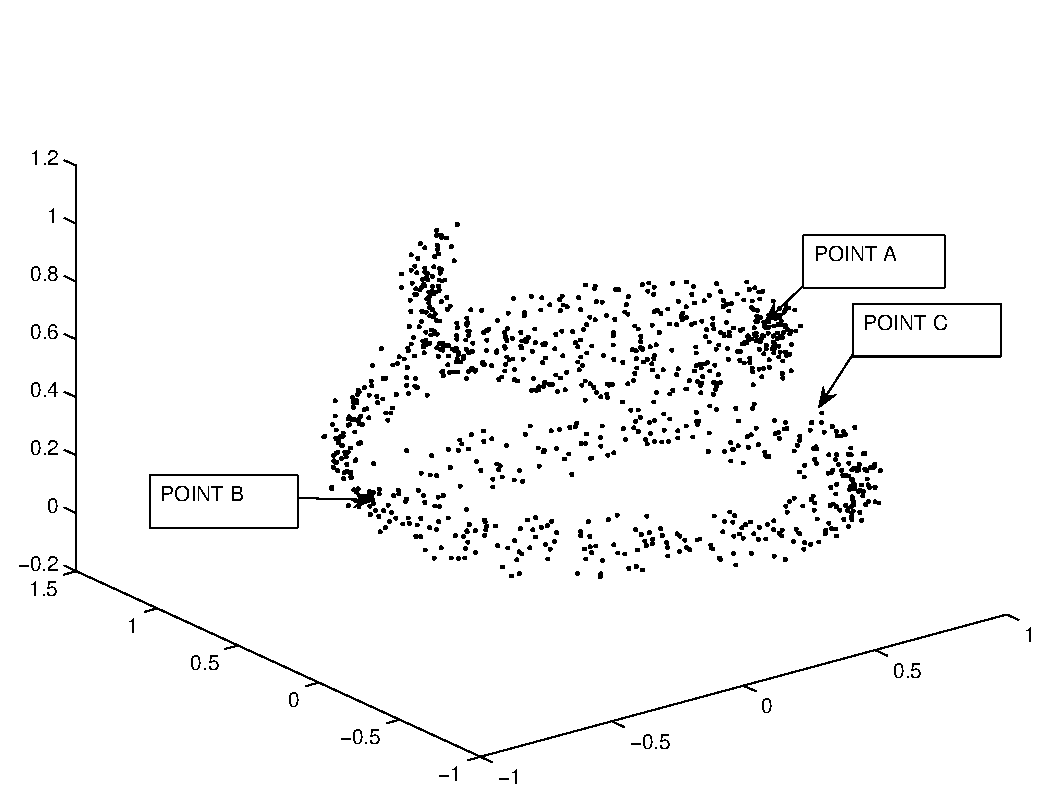
\includegraphics[width=\textwidth]{spiral.eps}
\end{figure}
\end{column}
\begin{column}{.5\textwidth}
\begin{figure}[!]
\centering
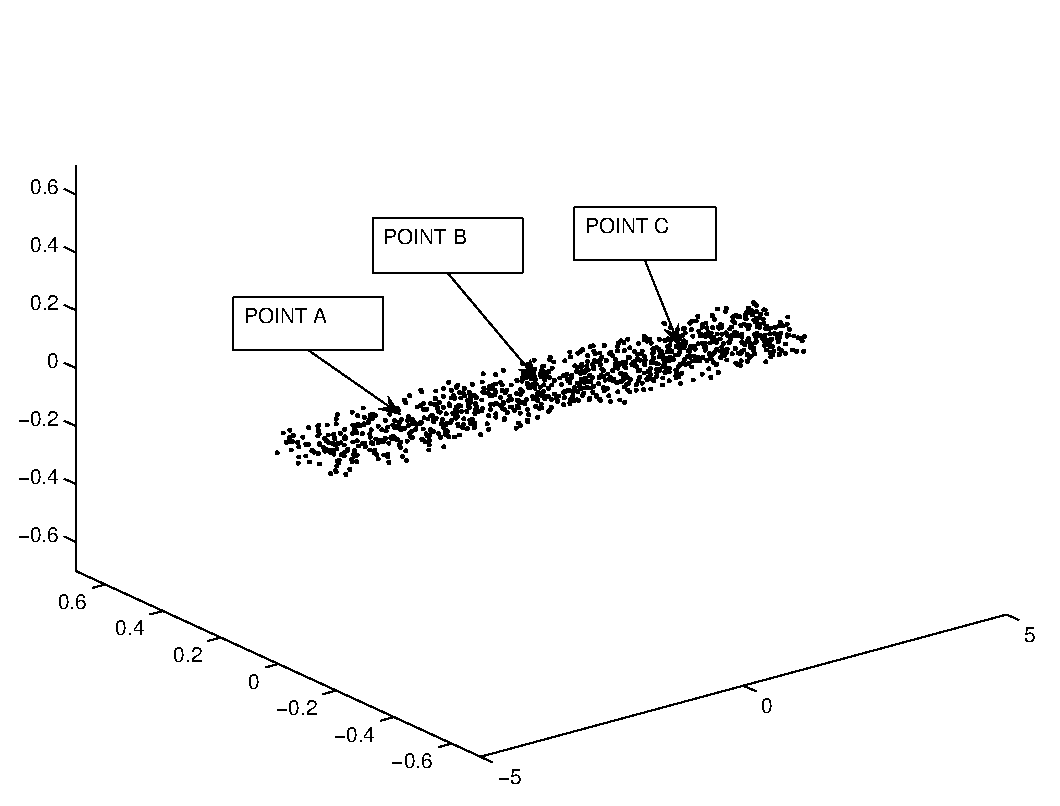
\includegraphics[width=\textwidth]{spiral2.eps}
\end{figure}
\end{column}
\end{columns}
\begin{itemize}
\item Better reductions are obtained by using increased depth and
nonlinearity.
\item Crucial to use nonlinear activations with deep autoencoders.
\end{itemize}
\vfill
\end{frame}



\begin{frame}{Recommender Systems}
\begin{itemize}
\item Recap of SVD: Factorizes $D \approx UV^T$ so that the
sum-of-squares  of residuals $|| D- UV^T||^2$  is minimized.
\begin{itemize}
\item Helpful to watch previous lecture on SVD
\end{itemize}
\item In recommender systems (RS), we have an $n \times d$ ratings matrix
$D$ with $n$ users and $d$ items.
\begin{itemize}
\item Most of the entries in the matrix are unobserved
\item Want to minimize $|| D- UV^T||^2$ only over the observed
entries
\item Can reconstruct the entire ratings matrix using $UV^T$
$\Rightarrow$ Most popular method in traditional machine learning.
\end{itemize}
\end{itemize}
\end{frame}


\begin{frame}{Difficulties with Autoencoder}
\begin{itemize}
\item If some of the inputs are missing, then using an autoencoder
architecture will implicitly assume default values for some inputs
(like zero).
\begin{itemize}
\item This is a solution used in some recent methods like {\em AutoRec}.
\item Does not exactly simulate classical MF used in recommender systems because it
implicitly makes assumptions about unobserved entries.
\end{itemize}
\item  None of the proposed architectures for recommender systems in
the deep learning literature  exactly map to the classical
factorization method of recommender systems.
\end{itemize}
\end{frame}


\begin{frame}{Row-Index-to-Row-Value Autoencoder}
\begin{itemize}
\item Autoencoders map row values to row values.
\begin{itemize}
\item Discuss an autoencoder architecture to map the one-hot
encoded row {\em index} to the row values. \item Not standard
definition of autoencoder.
\item Can handle incomplete values but cannot handle out-of-sample
data.
\item Also useful for representation learning (e.g., node representation of graph adjacency matrix).
\end{itemize}
\item The row-index-to-row-value architecture is not recognized as a
separate class of architectures for MF  (but used often enough to
deserve recognition as a class of MF methods).
\end{itemize}
\end{frame}


\begin{frame}{Row-Index-to-Row-Value Autoencoder for RS}
\begin{center}
\includegraphics[scale=0.83]{encoder3.eps}
\end{center}
\begin{itemize}
\item Encoder and decoder weight matrices are $U$ and $V^T$.
\begin{itemize}
\item Input is one-hot encoded row index (only in-sample)
\item Number of nodes in hidden layer is factorization rank.
\item Outputs contain the ratings for that row index.
\end{itemize}
\end{itemize}
\end{frame}


\begin{frame}{How to Handle Incompletely Specified Entries?}
\begin{center}
\includegraphics[width=.7\textwidth]{encoder4.eps}
\end{center}
\begin{itemize}
\item Each user has his/her own neural architecture with missing
outputs.
\item Weights across different user architectures are shared.
\end{itemize}
\end{frame}


\begin{frame}{Equivalence to Classical Matrix Factorization for RS}
\begin{itemize}
\item Since the two weight matrices are $U$ and $V^T$, the one-hot
input encoding will pull out the relevant row from $U V^T$.
\item Since the outputs only contain the observed values, we are
optimizing the sum-of-square errors over observed values.
\item Objective functions in the two cases are equivalent!
\end{itemize}
\end{frame}


\begin{frame}{Training Equivalence}
\begin{itemize}
\item For $k$ hidden nodes, there are $k$ paths between each user
and each item identifier. \item Backpropagation updates weights
along all $k$ paths from each observed item rating to the user
identifier.
\begin{itemize}
\item Backpropagation in a later lecture.
\end{itemize}
\item These $k$ updates can be shown to be {\em identical} to
classical matrix factorization updates with stochastic gradient
descent.
\item Backpropagation on neural architecture is identical to
classical MF stochastic gradient descent.
\end{itemize}
\end{frame}


\begin{frame}{Advantage of Neural View over Classical MF View}
\begin{itemize}
\item The neural view provides natural ways to add power to the
architecture with nonlinearity and depth.
\begin{itemize}
\item Much like a child playing with a
LEGO toy.
\item You are shielded from the ugly details of training by an
inherent modularity in neural architectures.
\item The name of this magical modularity is backpropagation.
\end{itemize}
\item If you have binary data, you can add logistic outputs for
logistic matrix factorization.
\item {\em Word2vec} belongs to  this class of
architectures (but  {\em direct} relationship to nonlinear matrix
factorization is not recognized).
\end{itemize}
\end{frame}


\begin{frame}{Importance of Row-Index-to-Row-Value Autoencoders}
\begin{itemize}
\item   Several MF methods in machine learning  can be
expressed as row-index-to-row-value autoencoders (but not widely
recognized--RS matrix factorization a notable example).
\item  Several  row-index-to-row-value architectures in NN literature  are also not fully recognized as matrix factorization
methods.
\begin{itemize}
\item The full relationship of {\em word2vec} to matrix
factorization is often not recognized.
\item {\em Indirect} relationship to {\em linear} PPMI matrix factorization was shown
by Levy and Goldberg. \item  In a later lecture, we show that {\em
word2vec} is {\em directly} a form of {\em nonlinear} matrix
factorization because of its row-index-to-row-value architecture and
nonlinear activation.
\end{itemize}
\end{itemize}
\end{frame}



\begin{frame}{Word2Vec: An Overview}
\begin{itemize}
\item {\em Word2vec} computes embeddings of words using  sequential
proximity in sentences.
\begin{itemize}
\item If {\em Paris} is closely related to {\em France}, then
{\em Paris} and {\em France} must occur together in small windows of
sentences.
\begin{itemize}
\item Their embeddings should also be somewhat similar.
\end{itemize}
\item Continuous bag-of-words predicts central word from context window.
\item Skipgram model predicts context window from central word.
\end{itemize}
\end{itemize}
\end{frame}


\begin{frame}{Words and Context}
\begin{itemize}
\item A window of size $t$ on either side is predicted using a word.
\item  This model tries to predict the context  $w_{i-t} w_{i-t+1}
\ldots w_{i-1}$ $w_{i+1} \ldots w_{i+t-1}  w_{i+t}$  around word
$w_i$, given the $i$th word in the sentence, denoted by $w_i$.
\item The total number of words in the context window is $m=2t$.
\item One can also create a $d \times d$  word-context matrix $C$ with frequencies
$c_{ij}$.
\item  We want to find an embedding of each word.
\end{itemize}
\end{frame}


\begin{frame}{Where have We Seen this Setup Before?}
\begin{itemize}
\item  Similar to recommender  systems with {\em implicit feedback}.
\item Instead of user-item
matrices, we have  square word-context matrices.
\begin{itemize}
\item The frequencies correspond to the number of times a  contextual word (column id) appears for a target word (row id).
\item Analogous to the number of units bought  by a user (row id) of  an item (column id).
\item An unrecognized fact is that skipgram {\em word2vec} uses an
almost identical model to current recommender systems.
\end{itemize}
\item Helpful to watch previous lecture on
recommender systems with row-index-to-value autoencoders.
\end{itemize}
\end{frame}


\begin{frame}{Word2Vec: Skipgram Model}
\begin{center}
\includegraphics[width=.4\textwidth]{word2vecskip.eps}
\end{center}
\vspace{-0.35in}
\begin{itemize}
\item Input is the one-hot encoded word identifier and output contains $m$ {\em identical} softmax probability sets.
\end{itemize}
\end{frame}


\begin{frame}{Word2Vec: Skipgram Model}
\begin{center}
\includegraphics[width=.4\textwidth]{word2vecbatch.eps}
\end{center}
\begin{itemize}
\item Since the $m$ outputs are identical, we can collapse the $m$
outputs into a single output.
\item  Mini-batch the words in a context window to achieve the same
effect.
\item Gradient descent steps for each instance are proportional to
$d$ $\Rightarrow$ Expensive.
\end{itemize}
\end{frame}


\begin{frame}{Word2Vec: Skipgram Model with Negative Sampling}
\begin{center}
\includegraphics[width=.4\textwidth]{word2vecbatch.eps}
\end{center}
\begin{itemize}
\item  Change the softmax layer into sigmoid layer.
\item  Of the $d$ outputs, keep the positive output and sample $k$
out of the remaining $d-1$ (with log loss).
\item Where have we seen missing outputs before?
\end{itemize}
\end{frame}


\begin{frame}{Can You See the Similarity?}
\begin{center}
\begin{tabular}{c}
\includegraphics[width=.4\textwidth]{seen.eps}\\
\includegraphics[width=.4\textwidth]{encoder3.eps}
\end{tabular}
\end{center}
\begin{itemize}
\item Main difference: Sigmoid output layer with log loss.
\end{itemize}
\end{frame}


\begin{frame}{Word2Vec is Nonlinear Matrix Factorization}
\begin{itemize}
\item Levy and Goldberg showed an {\em indirect} relationship
between {\em word2vec} SGNS  and PPMI matrix factorization.
\item We provide a much more direct result in the book.
\begin{itemize}
\item Word2vec is (weighted) logistic matrix factorization.
\item Not surprising because of the similarity with the recommender
architecture.
\item Logistic matrix factorization is already used in recommender
systems!
\item Neither the {\em word2vec} authors nor the community have
pointed out this {\em direct} connection.
\end{itemize}
\end{itemize}
\end{frame}


\begin{frame}{Other Extensions}
\begin{itemize}
\item We can apply a row-index-to-value autoencoder to any type of matrix to learn
embeddings of either rows or columns.
\item Applying to graph adjacency matrix leads to node embeddings.
\begin{itemize}
\item Idea has been used by {\em DeepWalk} and {\em node2vec} after
(indirectly) enhancing the matrix entries with random-walk methods.
\item Details of graph embedding methods in book.
\end{itemize}
\end{itemize}
\end{frame}







\begin{frame}
\frametitle[alignment=center]{}
\flushbottom
\centering
Thank you!\\
\href{mailto:tiago@ic.ufal.br}{tvieira@ic.ufal.br}\\
%\href{mailto:warley.barbosa@edge.ufal.br}{warley.barbosa@edge.ufal.br}\\
%\href{mailto:icaro.bastos@edge.ufal.br}{icaro.bastos@edge.ufal.br}\\
\end{frame}



\end{document}
